\section{System Architecture}

Chickenizer flows in one direction: rules and payoffs $\rightarrow$ validated strategies $\rightarrow$ engine $\rightarrow$ Nash and repeated analysis $\rightarrow$ payloads and optional UI. Figure~\ref{fig:arch} shows the main dependencies; dashed lines are optional (Streamlit, Q-learning helpers).

\begin{figure}[t]
  \centering
  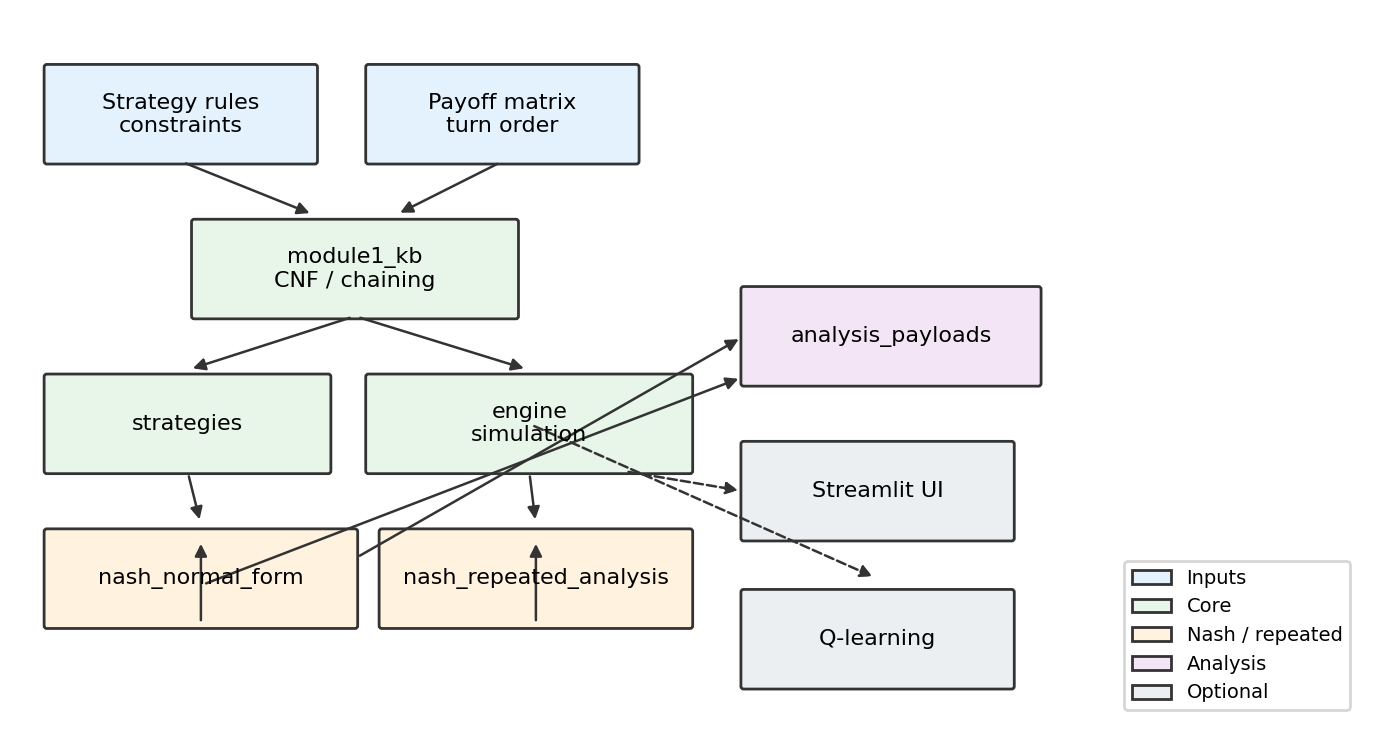
\includegraphics[width=0.95\linewidth]{figures/architecture.png}
  \caption{High-level data flow in the Chickenizer repository. Solid arrows: core library use; dashed arrows: optional UI and learning tools. Figure generated by \filepath{paper/scripts/gen_architecture_figure.py}.}
  \label{fig:arch}
\end{figure}

\textbf{Engine and strategies.} \texttt{GameEngine} holds state (actions, HP, resilience, reputation, preferences, histories, end reason). Strategies implement a shared interface in \texttt{strategies.py} and may use the knowledge base or hand-written rules. Each round updates resilience from merged preferences and checks stop rules (round cap, resilience gap, etc.). Analysis code often uses NumPy~\cite{numpy}.

\textbf{Nash (one-shot).} \filepath{nash_normal_form.py} fills a $2\times 2$ matrix by running one counterfactual round per cell from the current baseline so cells reflect resilience after that joint choice. Pure Nash is by best-response scan; mixed equilibria use Nashpy when needed. This stays separate from long multi-round runs.

\textbf{Repeated play.} \filepath{nash_repeated_analysis.py} runs many rounds with two fixed strategies and returns summaries (per-round log, action frequencies, resilience series, and averages grouped by the previous round's joint action). The code states clearly that this is not Nash equilibrium of the repeated game.

\textbf{Analysis and UI.} \filepath{analysis_payloads.py} bundles results for consumers including Streamlit under \filepath{.src/ui/}. Q-learning tournament and heatmap scripts add optional comparisons between learned policies.

\textbf{End-to-end flow.} A typical library path is: build or load strategies that respect Module~1 constraints; run the engine (Module~4) for traces; optionally call \filepath{nash_normal_form} (Module~3) on the current state to read off equilibria of the induced $2\times 2$ game; optionally call \filepath{nash_repeated_analysis} (Module~5) for long-run counts and paths; pass structured dicts or dataclasses into analysis payloads or the UI. Module~2 search logic sits inside engine/strategy calls rather than as a separate executable, but tests still treat those behaviors as part of the search story.

\textbf{Tests.} \filepath{integration_tests/} checks handoffs between modules (for example, search vs.\ Nash on small states, simulation feeding analysis). Together with Figure~\ref{fig:arch}, that gives a concrete picture of allowed dependencies.
